\chapter{导言}

\section{现代经济学思想的核心焦点}

人们可感知的\textbf{需求}通常是无限的,人类常常是\textbf{贪得无厌}的,然而资源
(经常被划分为土地、劳动、资本及企业家才能)却是\textbf{有限}的。为了解决稀缺性问
题,需要一种社会机制在无限的选择中间来分配有限的资源。其中的一个方面便涉及如
何\textbf{限制个人需要、增加资源供给}的意愿。

从历史上来看,人们曾经运用过四种机制来处理稀缺性问题。第一种机制,也是最古老的机
制是\textbf{强制方式},它流行于早期社会,今天仍然被使用着。第二种机制是\textbf{传
  统惯例},它强调根据以往的方式分配资源。随着文明的出现,产生了第三种分配资源的社
会机制即\textbf{权威},它所采取的形式是\textbf{政府和教会制度}。第四种分配资源的
社会机制则是随着时间不断发展起来的\textbf{市场}(当前主要资源分配机制)。……都有,
且运行过程也不是线性的……

\textbf{公平、公正与合理问题}就深埋在稀缺性问题中……资源分配机制决定谁得到资源。
谁得不到资源。

\subsection{现代经济理论的划分}

在现代经济思想中,与相对稀缺性相连的问题一般被划分为微观经济学与宏观经济学。微观
经济学考虑资源配置与收入分配问题,宏观经济学考虑经济体的稳定与增长问题。配置问题
(生产什么与如何生产)与分配问题(实际收入如何在社会成员间分配)一般归于微观经济
理论。

宏观经济学聚焦于经济体的稳定与增长,关注整体经济的总变量:收入与就业水平、价格总
水平、经济增长率等。

\section{我们研究经济思想史所采用的方法}

\subsection{相对论者的方法与绝对论者的方法}

相对论者的方法relativist approach和绝对论者的方法absolutionist approach

\textbf{相对论历史学家}们关心:(1)引起人们考察某些经济问题的\textbf{历史、经济、
  社会和政治力量}是什么;(2)这些力量塑造新型理论内容的方式。他们主张在每个经济
理论的发展过程中,\textbf{历史}都扮演着一定的角色。

\textbf{绝对论}经济学家(下文中有时称作辉格党(Whigs)强调内在力量如经济学中日益
盛行的\textbf{专业化},对经济理论发展的解释。绝对论者宣称,理论的进步不仅仅反映了
历史环境,而且取决于训练有素的专业人员对未决问题或似是而非观点的发现与解释……按
照这一观点,有可能\textbf{绝对地按照理论的价值进行排序};并且最新近的理论很可能存
在较少的错误,比较早的理论更贴近事实。

我们的观点……无论……都是不能令人信服的。应将经济思想史看成是学科的外在力量与内
在力量相互作用的动态过程,这些力量会产生新的理论。

\subsection{正统的经济学家与非正统的经济学家}

辉格党认为全部经济思想是\textbf{观念的演进},目标朝向现代思想的终场,可事实是终场
还远着呢……

非正统经济理论(heterodox economic theory)现代非正统流派中包括奥地利流派、制度
主义流派、后凯恩斯主义流派、激进主义流派,每一种流派都与主流分享一段历史。

现代正统理论家主要集中在\textbf{资源配置、分配、稳定与增长}这四个问题上,非正统经
济学家则研究\textbf{社会与经济中产生变化的力量}。正统经济学家认为具体的社会制度、
政治制度与经济制度是\textbf{既定}的(也就是他们没兴趣解释的那些事情),并在这些制
度背景下研究经济行为,非正统经济学家则聚焦于\textbf{导致这些制度演变的力量}。

非正统经济学家与正统经济学家的区别经常表现在所注意的问题上,而不是理论本身直接对
立上。

\section{非正统经济学家的角色}

\section{呈现思想多样性时的问题}

\section{方法论问题}

\subsection{作为一门艺术与作为一门科学的经济学}

经济思想中最重要的区别也许是\textbf{经济学艺术}(the art of
economics)、\textbf{实证经济学}(positive economics,也称经济学科学)
与\textbf{规范经济学}(normative ecnomics)之间的区别。

实证经济学所关心的是\textbf{支配经济活动的力量}。它会问诸如此类的问题:经济体是怎
样运转的?决定收入与分配的力量是什么?这些询问的唯一目的是为了了解而了解,处理经
济变量之间实证的、事务性的关系,经常表述为“\textbf{是什么}”。规范性的判断应当尽
可能少地进入分析。规范经济学明确地关注\textbf{应当怎样}的问题。它是经济学的哲学分
支,使\textbf{经济学与道德}相结合。经济学艺术关注\textbf{政策问题}。它将经济学的
科学性(是什么)与规范经济学(应当怎样)\textbf{联系}起来,提出如下问题:如果这些
是一个经济体的规范性目标,并且如果这是经济体运转的方式,那么,这个经济体怎样才能
最好地实现这些目标?

实证经济学、规范经济学和经济学艺术三者之间的区别是很大的……完全不同的方法……实
证经济学的方法是\textbf{形式化的、抽象的};它试图将经济力量与政治和社会力量区分开。
经济学艺术的方法更加复杂,因为它关注\textbf{政策},而且必须致力于政治社会力量与经
济力量相互关系的研究。在经济学一书中,必须给从实证经济学中抽象出来的问题添加所有
的维度。

\textbf{德国历史学派与英国马歇尔学派}都提倡,主要的精力应当放在\textbf{经济学艺
  术}上。他们从亚当·斯密的著作中汲取力量来拥护这一主张。现代正统经济学家则集中于
实证经济学,在大卫·李嘉图的著作中为其立场寻找支持……我们在本章附录中对方法论的讨
论也将遵循这一焦点。然而,当我们考察不同经济学家提出的经济政策时,我们将回到经济
学艺术中很多有趣的问题上。

\subsection{经验验证的重要性}

就像科学方法中所力证的那样,成长中的科学界努力发现真理时所借助的手段,包括经过专
门训练的经验观察。这使得推理与经验观察的综合成为必须。……我们将简单地界定在讨论
中其重要作用的三个术语,即\textbf{归纳的}(inductive)、\textbf{演绎
  的}(deductive)及\textbf{溯因的}(abductive)方法。

溯因法把历史、制度与经验研究结合在一起,以获得真理;然而,它并不声称提供了一个权
威性的理论,因为当我们处理一个复杂的系统时,权威性的理论会超越我们的领会。

\section{从经济思想史研究中获得的益处}

\section{本章扩展内容}

\subsection{经济学专业及其方法}

经济学的专业化只是在最近一百年中才发生的。即使我们采取较为宽泛的观点,将经济学视
为一门知识学科,它也仍然相对年轻。1500年之前,没有什么群体专门去了解经济学。

从1776年至1876年的这段时期,见证了政治经济学学科的日益专业化。

到了1900年,政治经济学有了一个新的名称:经济学(economics),并且作为一门美国和
欧洲大学的课程。

\subsection{经济学思想的传播}

“\textbf{发表还是毁灭}”统治着残酷竞争的学界。

\subsection{方法论思想的演进}

\begin{enumerate}
\item \textbf{逻辑实证主义}的兴起。1920年代后期由维也纳学派发起,将演绎推理与实证
  主义家让事实为自己辩护的愿望连接起来。

  逻辑实证主义家认为,科学家发展了一种演绎结构(一种逻辑理论),产生了在经验上可
  以验证的命题。\textbf{然而,只有当一种演绎理论在经验上被检验与核实之后,它才能
    被认同是正确的。}

  正是逻辑实证主义使规范经济学与实证经济学之间的区别形式化……规范性的论述不符合
  这一科学方法……

摘自
\href{https://zh.wikipedia.org/wiki/%E9%80%BB%E8%BE%91%E5%AE%9E%E8%AF%81%E4%B8%BB%E4%B9%89}{维基}:
  \begin{quotation}
    对逻辑实证主义的批评:对于从感官经验知识得来的知识,逻辑实证主义不能给出一个
    满意的描绘。这同过去的激进经验主义面临的问题是一样的。逻辑实证主义取决于如此
    服务于科学的逻辑:\textbf{某个具有特殊威信的证实理论。然而最终谁也没能提出这
      样的理论。}
  \end{quotation}


\item 从逻辑实证主义到\textbf{证伪主义}。波普尔在20世纪30年代提出,经验检验并不能确定一种
  理论的真相,只能确定假象,这就是为什么波普尔的方法有时被称为证伪主义
  (falsificationism)的原因。根据\textbf{波普尔}的观点,\textbf{根本没有可能性
    来“证实”一种理论,原因是人们不可能完成理论的所有可能性检验。}……理论预言结
  果的发生,只能表明理论\textbf{尚未被证明}是错误的。……下一次实验可能会产生与理
  论预言不一致的错误。

\item 从证伪主义到\textbf{范式}。对波普尔理论的现代否定:\textbf{一些理论的检验预
    言并不能得到检验;难以决定理论被证伪或没有被证伪。}例如,检验程序缺陷、外在因
  素;研究者的心态,研究者未能检验已确立理论的含义,便假定理论的含义是正确的,主
  观错误。

  \textbf{托马斯·库恩《科学革命的结构》}。\textbf{范式是一种既定的方法以及构成研
    究者分析组成部分的知识体,它遵循着任何既定时期所公认的对主流科学思想的教科书
    陈述。}库恩认为,大多数科学研究是\textbf{规范科学}(normal science),研究者
  试图解决在现有范式的框架内所提出的难题。这一研究经常使得范式\textbf{未能说明的
    不规则现象}频繁出现,但是,这种不规则的存在还不足以颠覆占统治地位的范式……一
  旦这样一种出众的范式得到发展,一场科学革命就成为可能。

  占优势地位的理论不一定是最好的理论

\item 从范式到\textbf{研究纲领}。伊姆雷·拉卡托斯(Imre Lakatos),\textbf{现有理
    论可能并不包含真理}。……他观察到科学家们从事发展竞争性研究纲领时,每个研究纲
  领不仅包含对一系列的数据进行分析和证伪,而且包含无可非议地接受一系列
  的\textbf{硬核逻辑假设}。每项研究都\textbf{从硬核中得出一组周边假设},然后试图
  对它们进行\textbf{证伪}。对某一个周边假设的证伪并不要求放弃理论,但是会引起对逻
  辑结构的重新考虑或调整。只有当“\textbf{足够多}”的周边假设被证伪时,硬核假设才
  被重新考虑。如果对周边假设进行证伪的过程继续进行,拉卡托斯就将研究纲领称作
  是\textbf{进步的},否则被称作\textbf{退化的}。拉卡托斯的研究有两个重要特征:
  (1)承认证伪过程的复杂性;(2)早期的分析要求某一种理论成为主流,拉卡托斯则提
  出多种可利用理论同时存在。

  摘自 \href{https://zh.wikipedia.org/wiki/%E7%A0%94%E7%A9%B6%E7%BA%B2%E9%A2%86}{维基百科}:
    \begin{quotation}
      拉卡托斯提出的研究纲领是由一个稳定、不容改变的“硬核”(hard core)与一个允
      许调整以应对批评的“保护带”(protective belt)构成的。拉卡托斯认为,科学发
      展的模式即是不同科学研究纲领间动态变化的过程。当调整一个研究纲领的保护带已
      不足以预见新的事实以及解释以往的事实时,这个纲领变由进步的变为退步的,并会
      被新的进步的研究纲领所取代。而退步的研究纲领也可能在以后卷土重来,重新成为
      进步的纲领。
    \end{quotation}

\item 从研究纲领到社会学方法与修辞方法。从某一方面来看,我们上面所描述的发展越来
  越多地远离逻辑实证主义,但是从另一方面来看,认识到经验检验的局限性又是对逻辑实
  证主义的完善与改进。

  \textbf{保罗·卡尔·费耶阿本德(德语:Paul Karl Feyerabend)《反对方法:无政府主
    义知识论纲要》。}对任何方法的认同都限制了解决问题的创造力,因此,最好的科学只
  限于\textbf{没有方法的科学}——换个说法,\textbf{一切尽随其变}。尽管他的激进观点
  最初看上去很疯狂,然而,就阐明修辞方法与社会方法只是来说,他提出了一些新的观点,
  影响了经济新方法近来的发展。

  因为它们拒绝假设存在终极的、神圣的真理,所以,它们便找到其它理由来解释为什么人
  们相信他们所相信的。

  方法论中的\textbf{修辞方法(rhetorical approach)强调语言的说服力}。该方法主
  张,\textbf{一种理论之所以被接受,不是因为它本来就是正确的,而是因为理论的提倡
    者借助他们出众的修辞,成功地使其他人相信理论的价值。社会方法考察社会与制度约
    束,这些约束影响着对一种理论的认可。资金、职业、媒体的控制……}

\item \textbf{后修辞学方法}。混乱……极端观点,\textbf{最善言辞的研究者赢得胜利},
  而无视其研究价值的大小。

  后修辞学方法(postrhetorical methodology),将费耶阿本德的见解与更加切实可行的
  方法相结合,并且\textbf{强调溯因胜过演绎与归纳}。……后修辞经济学家将会仔细调
  查\textbf{研究者研究特定理论的动机},以\textbf{怀疑论}来看待与研究者自身利益或
  预想观点相符合的研究结果,“\textbf{让每一朵花儿绽放}”。最后,与逻辑实证主义者
  或证伪主义者相比,后修辞经济学家将非常有可能遵循贝叶斯统计而不是古典统计。

  \textbf{贝叶斯主义者}(Bayesians)认为,人们能够发现语句中更高级或更低级的真理,
  但不是终极真理。贝叶斯的影响将会造成对古典统计检验的重新解释,致使它们不太精确,
  不太有说服力,不能独立代表某一具体置信水平。在未来的方法论中,关于研究者以及研
  究信息,将有可能成为统计报告中的一个必要组成部分。

\end{enumerate}

\part{前古典经济学}

回顾这些前古典经济学家时,重要的是记住两点。第一,他们只是说出了经济体有限的方面,
并没有将他们的分析扩大到一个全面的经济系统中。……第二,发生在几个世纪中的经济思
想的变化,部分地反映出社会经济结构的变化。例如,在\textbf{英国},\textbf{经院哲学
  经济思想}源自于\textbf{封建主义},而\textbf{重商主义理论}则源自于\textbf{商业资
  本主义}。出现在自由重商主义著作中的古典自由放任观点,也与生产者资本主义的萌芽有
联系。

\chapter{早期前古典经济思想}

本书将公元前800年到1500年划分为早期前古典阶段,将1500年至亚当·斯密《国富论》出版
的1776年划分为前古典时期。

我们将早期前古典阶段(preclassical period)划分为四个分阶段:(1)早期东方经济思
想,管子(公元前725--前645)为代表。(2)希腊思想,赫西俄德(公元前800年)《工
作与时日》、色诺芬(公元前435--前355)《增加雅典国家收入的方法》、亚里士多德《政
治论》为代表(3)阿拉伯--伊斯兰思想,安萨里(1058--1111)、伊本·赫勒敦(1332--1406)
(4)托马斯·阿奎那《神学大全》。

\section{一些粗略的概括}

现代经济理论认为,所有经济问题的源泉都是相对稀缺性,注意力集中在市场。早
前\textbf{前古典经济学思想家}不像现代经济学家那样特别关注资源配置的效率,他们是为
了\textbf{公平与生活质量}而去考虑不同类型经济活动的结果。

两个重要主题从早期前古典学说中显露出来。第一个主题涉及用来分析社会的研究层
面。\textbf{这一类经济学家认为,将任何一种特定的活动——如经济活动——与其他活动相分
  离是不合适的。}

第二个主题是关注一些粗略的哲学问题,尤其是关注合理、公正与公平问题。

\section{非西方的经济思想}

《管子》,远远超越了公共事务管理的墨子。书中包含属于经济思想核心的很多观点,其中
最重要的可能是他的“轻/重”理论,它可以被视为是对供给、需求理论的语言。其他还包
括他对数量理论的语言、对反周期财政政策的讨论,以及市场运转的语言。

趋利避害……物品和货币的轻重(物品充裕则轻,价格下跌。物品“锁藏”则重,价格下
跌……货币重指货币价格上涨,产品价格下降;货币轻指货币价格下降,产品价格上升)。
为阻止这种波动,他建议国家在货币重时购买商品,货币轻时卖出商品。这不仅有助于稳定
价格水平,而且还能为政府赚钱。

\section{希腊思想}

赫西俄德《神谱》,稀缺性并不起因于和有限资源及无限欲望相关的人类环境。更合适的解
释是:它是当潘多拉打开魔盒时所释放的\textbf{邪恶之一}。赫西俄德是个农场主,对效率
很感兴趣。

早期经济学家因对稀缺性及其含义,以及对经济体的概念还不具备真正的洞察力,所以对社
会层面的效率问题不感兴趣。源自于希腊语的经济学一词,被色诺芬作为《经济论》这本书
的题目而使用……希腊人所使用的这一术语,是指\textbf{生产者与(或)家庭层面的有效
  管理}。色诺芬在著作中采用了有效管理的概念,并且在\textbf{家庭、生产者、军事、公
  共事务}层面上使用了这一概念。

\subsection{亚里士多德}

\textbf{德谟克利特}不仅主张\textbf{劳动分工},而且认为\textbf{财产私有权}作为一种
动力,会导致更多的经济活动。\textbf{柏拉图}《理想国》中认为武士与哲学家——其理想国
中的统治阶级,不应当拥有\textbf{私人财产}(private property),但是应当掌
控\textbf{公共财产}(communal property),以\textbf{避免对财产的争夺},这种争夺会
将他们的注意力从更重要的事情上展开。然而,\textbf{亚里士多德}认为私人财产在社会中
发挥着有益的作用,\textbf{不应当制定规则来限制}私人手中的财产数量。它一方面是谴责
追求经济利益的行为,同时又认可拥有私人财产的权利,这种\textbf{明显的矛盾}在16世纪
之前,一直使道德哲学家们感动苦恼。

亚里士多德对经济思想的主要贡献涉及\textbf{商品交换与交换中货币的使用}。他
说,\textbf{人们的需要是适度的,但人们的欲望是无限的。}因此,\textbf{满足需
  求}(needs)的商品生产是恰当与正常的,但是,力图\textbf{满足无限欲望}的产品生产
就是不正常的。……很难确定生产出售活动是在满足需要还是在满足过度欲望;但是他假定,
如果市场交换采取\textbf{物物交换}的形式,活动的目的就是\textbf{满足正常需要},并
且不存在想要的经济利益。但是使用\textbf{货币作为媒介},就表明交换的目的
是\textbf{货币收益},这是亚里士多德所谴责的。

亚里士多德提出的令人关注的论点之一是,通过减少消费改变人们的态度,来对待稀缺性问
题。对于各种乌托邦人士和社会主义者来说,这是一个有力的论点,他们希望通过排除稀缺
性固有的冲突来结束社会冲突。

\section{阿拉伯--伊斯兰思想}

众所周知,希腊思想被翻译成拉丁文,是为了供来自拉丁语而非希腊语的经院哲学使用。在
很多学科中,阿拉伯人做出了属于自己的重要贡献。

现代经济学家是从整个人类生活的角度来提炼经济活动的,尤其是21世纪……然而,阿拉
伯--伊斯兰经济学家出于拯救的缘故去考虑人类活动的所有方面,尤其是活动的后果。

征税

在较重要的阿拉伯--伊斯兰经济学家中,正式提出经济问题的是艾布·哈米德·安萨里与伊本·赫
勒敦。

\subsection{艾布·哈米德·安萨里}

他关于市场通过自愿交换不断演进的描述,对于一个11世纪的创作者来说,是非常有洞察力
的。他关于随着专业化和劳动分工的发展,市场如何连接与调整经济活动的见解也是如此。

安萨里观察到,在他所处的时代,一个面包可能是一千个甚至更多工人的产品。认识到越
来\textbf{越多的专业化与劳动分工导致经济交换,安萨里暗示了物物交换的困难,以及随
  之发生的对货币的需要,货币便利了交换。}他也考察了许多其它的经济话题:\textbf{公
  共支出、征税与借贷、制造硬币与降低硬币价值、利息与高利贷},以及如何更好地征税,
以便适当地在全社会分散税务负担。

\subsection{伊本·赫勒敦}

他对经济问题最令人注目的见解,可能起因于对如下问题广泛而彻底的考察,即他的国家怎
样具有今天所称的发展周期,从低收入、低工艺技能以及少量经济剩余的\textbf{农村沙漠
  生活社会},演变为劳动生产率和收入、经济剩余、人口增长都较高的\textbf{农业占优势
  的非游牧社会}。以今天的观点来看,我们能看到伊本·赫勒敦所考察的很多经济话题:人
口、利润、供给、需求、价格、奢侈品、总剩余、资本构成。

\subsection{需求与欲望}

按照\textbf{现代正统理论家}的观点,在市场经济中,\textbf{区分需求与欲望在客观上是
  不可能的}。他们感到,亚里士多德所奉行的准则应当被视为是与其时代相应的指导方针,
但并不适合于我们的时代,因为他们与现今的经济现状不协调。……人是否\textbf{合乎道
  德}地从事产品生产与交换,应当\textbf{最终留给个人去决定}。但是,很多非正统流派,
例如\textbf{制度主义者},不赞同这一立场。…… \textbf{需求能够并且一定要与欲望区
  分开来}。

\section{经院哲学}

经院哲学时期从罗马帝国衰落之前开始,到重商主义在西欧开始时结束。

\subsection{经院哲学思想的封建基础}

尽管供市场销售的产品生产,在整个中世纪得到增加,但是它并没有在日常生活中扮演支配
角色。\textbf{封建经济由社会中的自给农业组成,不是依靠市场而是依靠惯例、习俗与权
  威来维系社会。}社会被分为四个集团:奴隶、地主、皇室及牧师。全部土地基本上归罗马
天主教教会或国王所有。地主或贵族享有土地使用权并可以世袭,并履行对应的义务。

\textbf{每个领地或庄园都是一个几乎完全的经济与政治单位,通常有自己的教堂。}教堂由
地主兴建,并由地主任命牧师。……一般来说,与封建庄园相比,领地都得到了较好的管理,
这在一定程度上是因为牧师是唯一精通阅读与写作的阶层。

\textbf{全部土地都属于上帝},上帝或者将土地交给\textbf{君权神授}的国王;或者交给
教会掌管。如果一个人不承认其上级的权威,就是与上帝的意愿相对立,因为上帝赋予了他
们权威,这个人\textbf{下辈子的救赎}就会受到危及。

大部分经济史学家将技术的变化视为封建主义衰老的主要原因。农业技术变革对领地的影响
足以造成混乱。来自水和风的机械力取代了人力和畜力,基于此,制造业开始启动。

中世纪学派提出的道德问题今天也是切题的。从最宽泛的角度来看,我们仍然要问自己“美
好生活”是由什么构成的。……中世纪教会所担心的是,越来越多的经济活动,将把人类的
智力与心灵,从对宗教和道德的关注转向物质享乐主义。

经院哲学关注价格体系中的公正或公正缺失,它适用于当今的社会与经济体系。

\subsection{托马斯·阿奎那}

经院哲学实质上提出的还是同样的核心经济问题:私有财产制度以及公平价格与高利贷的概
念。……它努力调和教堂的宗教教义与当时慢慢增加的经济活动。

托马斯·阿奎那的重要性在于,他融合了宗教教义与亚里士多德的著作,这位经院哲学经济学
说提供了大量内容。他不得不对《圣经》中谴责私人财产、财富以及追求经济利益的大量相
关内容作出判断。依据《新约圣经》,\textbf{早期基督教思想认为公共财产符合自然法则,
  私人拥有的财产不符合这一理想。}……\textbf{早期经院哲学经院哲学经济学家}长期努
力地去证实,普通教徒的私人财产权与宗教教义\textbf{并不矛盾}。

\textbf{阿奎那}改变了亚里士多德的思想,因此他能够有说服力地指出,私人财产并不违背
自然法则。尽管他承认在自然法则下,所有的财产都是公共性的,但他坚持认
为,\textbf{私人财产的增长是对自然法则的一种补充,与之不矛盾。}

\begin{quotation}
  我们可能会说,对人类来说裸露身体是符合自然法则的,因为自然没有给予他衣服,但是
  技术发明了衣服。在这个意义上,占有所有东西……可以说成符合自然法则,因为占有上
  的差别……不是自然带来的,而是人类为了生活利益设计出来的。《神学》p47。
\end{quotation}

再次仿效亚里士多德,阿奎那\textbf{赞成由国家制定私人财产规则,并认可私人财产的不
  平等分配。}然而,遵循柏拉图的精神,阿奎那仍然提倡对那些坚定投身于宗教的人来说,
短缺与公共生活是一种理想状态,原因在于公共生活能够使他们将最多的经历专门用于宗教
活动。

阿奎那断言,当市场上发生交换行为以适应贸易各方的需要时(亚里士多德关于需求的概
念),不会涉及道德问题。但是,当个人抱有收益预期而为市场生产时,\textbf{只有当他
  们的动机是仁慈的时候,他们的价格才是公正的,他们的行为才是合乎道德的。}

\begin{quotation}
  用高利贷的方式把钱借出去,本身就是不公正的,因为这是在出售并不存在的东西,并且
  会不可避免地导致与公正相反的不平等。
\end{quotation}

一些经济理论史家主张,包括阿奎那在内的经院哲学\textbf{将公正价格视为劳动成本的对
  应词}。其他人则说它是\textbf{效用的对应词},还有一些人将它视为\textbf{生产总成
  本的对应词}。因此,经院哲学的公正价格概念也可以有选择地被堪称是下面这些理论或观
点的先驱,即李嘉图--马克思劳动价值理论、边际效用观点,以及古典--新古典理论中所暗
示的竞争性市场产生理想公正价格的观点。另一种被广泛持有的观点,是将经院哲学公正价
格概念视为能够\textbf{保持封建主义等级}的一组社会经济力量中的一个完整组成部分。该
主张认为,如果市场上的所有价格都是公正价格,那么,没有人能够通过经济手段改变他或
她的社会地位。经院哲学中经济分析的缺失,使其难以准确判断“公正价格”意味着什么。

在经院哲学学说中高利贷具有《圣经》上的以及亚里士多德式的意义,即任何获益行
为。……\textbf{《圣经》对高利贷的谴责,源于强者利用弱者这一风险。}此
外,\textbf{亚里士多德}提出通过借贷而获益是不正常的,因为\textbf{货币是不生殖的}。
从早期对获益相当严格的禁止到后来的接受——至少为了商业目的、经院哲学的观点逐渐得以
缓和。

\chapter{重商主义、重农主义及古典经济思想的其他先驱}

1600年至1750年,这150年间的特点是经济活动的增加。在经济上、社会上、政治上自给自
足的封建主义领地,正在给越来越多的贸易、领地外城市的增长,以及单一民族国家的成长
让路 。个人的活动更少受控于封建社会的习俗、惯例以及教会的权威。为市场而进行的产
品生产变得越发重要,并且土地、劳动、资本开始在市场上被购买与销售。这些都为工业革
命奠定了基础。

在这一时期,经济思想从简单的关于个人、家庭、生产者的观点,向更复杂的将经济体视为
其自身规律与相互关系的一个系统的观点演进。

\section{重商主义}

经院哲学的经济文献出自中世纪牧师之手,\textbf{重商主义的经济理论则是商人的杰作}。
他们创作的文献集中于经济政策问题上,通常与商人经济学家试图推动的某一\textbf{利益
  相关联}。

\subsection{每个人都是他自己的经济学家}

重商主义时代每位经济学家都倾向于主攻一个主题,没有哪一个经济学家能够令人印象深刻地
综合这些贡献。

\subsection{权力与财富}

可以将重商主义最准确地理解为,它是对当时问题做出的智力反应。重商主义时期,领地减
少,单一民族国家增多,\textbf{重商主义者试图确定能够推动国家权力与财富增加的最佳
  政策}。

重商主义者是在\textbf{世界总财富固定不变这一假设下}着手进行研究的。经院哲学利用相
同假设已经推断出,当贸易发生在个人之间时,\textbf{一个人所获得的必然是另一个人所
  失去的}。重商主义者将这一推理应用于国家之间的贸易,得出结论说一国财富与经济权力
的增加,是在损害其它国家财富与权力的情况下实现的。因此,重商主义者强调国际贸易是
增加一国财富与权力的一种手段,并且特别集中研究国家之间的贸易平衡问题。

根据大多数重商主义者的观点,经济活动的\textbf{目的是生产}——不像古典经济学后来主张
的那样是消费。……他们提倡通过同时\textbf{鼓励生产、增加出口、以及抑制国内消费}来
增加国家财富。因此,\textbf{一个国家的财富是依靠很多国家的贫困来支撑的}。尽管重商
主义者把很大精力放在生产上,但是却认为一个国家内部产品的大量供给是不合需要的。伴
随低水平国内消费的高水平生产,使得出口增加,这将会增加国家的财富与权
力。……提倡\textbf{低工资}……

\subsection{贸易平衡}

为了实现所谓的\textbf{贸易顺差},一个国家应当通过\textbf{关税、配额、津贴、税
  收}等手段来\textbf{鼓励出口,限制进口};应当通过政府干预国内经济,以及通过对外
贸易规则来刺激生产;应当对从国外进口的制造业产品征收保护性关税;应当鼓励进口用于
制造出口产品的廉价原材料。

重商主义者对贸易平衡(balance of trade)的特性与意义的看法不一致。

许多早期重商主义者\textbf{不是}根据一个国家的\textbf{产品生产量或者消费量}来界定
财富,而是根据\textbf{贵金属的拥有量}来界定财富。他们赞成贸易顺差,原因在于它将导
致贵金属流入国内经济以达成贸易平衡。

后来很多的重商主义者指出,只有将所有国家考虑在内的总体贸易平衡才是有意义的。如果
为出口产品所进口廉价原材料,那么暂时的贸易逆差和金银出口会导致总体贸易平衡的
改善。

\subsection{货币与重商主义}

重商主义文献的一个主要特点是,深信\textbf{货币因素}(monetary factors)而非实际因
素是经济活动与经济增长的首要的决定因素。他们相信,货币数量的变化引起了实际产量水
平——布匹码数与谷物蒲式耳数的变化。

亚当·斯密与古典经济学主张,经济活动的水平与经济增长率依赖于很多实际因素:劳动的数
量、自然资源、资本品、制度改革。\textbf{古典经济学家断言,货币数量的任何变化,既
  不影响产量水平也不影响增长水平,只影响价格总水平。}

\subsection{重商主义的现代分析}

凯恩斯在《通论》中认为,重商主义者对于促进经济发展的可行性政策已经有了深刻的了解。
但是,亚当·斯密与古典经济学家,以及从1776年至凯恩斯时期的历代正统经济思想家们,则
很少在大部分重商主义文献中发现什么优点。……斯密与其他古典经济学家强调决定产量水
平的世纪因素,他们的理论几乎专门集中于\textbf{供给}方面。而凯恩斯强调\textbf{总需
  求}的作用。…… 凯恩斯赞成重商主义者关于消费不足的观点,宣称他们关于增加货币数
量将会使产量增加的想法是合理的。凯恩斯说,重商主义者主张贸易顺差将增加国内支出,
并因此提高收入与就业水平。

一些对重商主义的评论,仔细而彻底检查的不是其支持者的观点,而是他们的动机。用现代
经济学的行话来说,重商主义者是“\textbf{寻租者}”。他们被利益动机所驱使,利用政府
为他们自身获取经济特权。他们通常都是商人,支持政府准许\textbf{垄断},以使商人垄断
者能够索要比没有垄断特权时更高的价格。


\subsection{重商主义者的理论贡献}

重商主义阶段后期,经济分析质量的提高相当显著,以至于这一时期被描述为包含着科学的
经济学的过渡时期。

\textbf{后期重商主义者}最重要的成就或许是清楚地认可了对经济体进行分析的可能性。这
一发展代表了当时自然科学中普遍存在的向社会科学的转变。\textbf{因果分析法替代了经
  院哲学的道德分析法}(并不代表与过去完全决裂)。但是,认为解释\textbf{自然规
  律}的方法同样能用来发现经济规律的观点,标志着持续发展的经济理论向前迈出了重要一
步。

此时对因果关系的认识机械。重商主义者中的一些人也正确地推论出,\textbf{低于均衡价
  格的最高限价将导致超额需求与短缺}。后期重商主义者在激励经济活动时,常常运用经济
人与利益动机的概念。他们说,政府不能改变人类的根本天性,尤其是他们以自我为中心的
驱动力。政治家将这些因素视为既定,试图形成一套法律与制度来引导这些驱动力,以期增
强国家的权力与繁荣。

很多后期重商主义者已经开始认识到他们的先驱所犯的严重的分析错误。例如,他们认识
到\textbf{货币并不是一个国家财富的衡量标准};对所有国家来说,不可能存在一种贸易顺
差;\textbf{没有一个国家能够长期保持贸易顺差;贸易可以互惠于各国;实行专业化与劳
  动分工的国家将具有优势。}越来越多的经济学家提出减少政府干预的数量。因此,重商主
义文献中包含早期古典自由主义的观点。

然而,没有一位前古典经济学家能够对市场经济的运行——价格的形成与稀缺资源的配置方式
提出完整的观点。重商主义者相信,\textbf{私人利益与公共福利之间存在根本的冲突}。因
此,他们认为,\textbf{对于政府来说有必要将私人的自我利益引导到公共利益上来}。古典
经济学家则在系统中找到了基本的协调,将公共利益视为个人追求自我利益自然而然的结
果。

\section{古典经济思想的影响力先驱}

\subsection{托马斯·孟}

他是东印度公司的一名董事,斯密认为他是最主要的重商主义者。

美国学生是在对美洲殖民地历史的了解过程中,间接获得有关重商主义理论与实践知识的。
英国政策的设计目的就是为了使殖民地成为原材料出口经济体,并依赖于英国的制造业产品。

托马斯·孟提出了重商主义的典型观点,但反驳那些包含批评东印度公司观点的较为原始的重
商主义观点。他指出,尽管与所有其他国家实现了\textbf{贸易顺差是合意的},贵金属流出
到所有其他国家是不合意的,但是,\textbf{与印度的贸易逆差以及出口贵金属到印度却有
  益于英国},因为这些实践扩大了英国与所有国家的贸易平衡,增加了金银的流入。

\subsection{威廉·配第}

\textbf{配第是第一个提倡测量经济变量的经济学家},出身贫寒,最终以一个有钱人的身份
终结一生。他的经济著作不是普通的论文,它们都源于配第在实践中感兴趣的事件,例
如\textbf{征税、政治、货币、度量}。

配第受到广泛的哲学运动的影响,这些运动发生在他出生之前和他在世期间。亚里士多德与
经院哲学几乎全用文字来阐述他们的论点,但是笛卡尔、霍布斯、培根使用归纳法、经验论
和数学受到了智力群体的关注。

配第提出应当使用数字、重量以及尺度术语来表达观点,应当只接受本质上具有明显基础的
论文,这种开创性见解是经济学现代思想的基石。尽管配第对统计学的早期应用显得有些原
始……

\subsection{伯纳德·曼德维尔}

他使用与众不同的活泼的语言与思想,以一种寓言诗的形式传达信息。《蜜蜂的寓言:私人的
恶习,公众的利益》不仅激怒了他同时代的人,而且也持续不断地使文学、哲学、心理学以
及经济学的学生意兴盎然。

他的讽刺诗抨击了所谓的感情脆弱的道德家……道德并不是用纯粹理性的原理制
成。\textbf{曼德维尔认为自私是一种道德恶习,但是如果自私的举动被政府适当地加以引
  导是能够产生社会利益的……}他发现世界是邪恶的,但仍主张“\textbf{在一个熟练政治
  家的灵巧管理下,私人恶习有可能变成公众利益。}”

\textbf{重商主义的信仰具体变现为对产品的恐惧,对生产过剩与消费不足的关注。}个人储
蓄并不受欢迎,因为它会引起更低的消费、更低的产量以及更低的就业。但是,就当时和现
在的很多人来说,储蓄是一种美德而支出则是一种恶习。曼德维尔嘲笑他们。

\textbf{曼德维尔主张拥有大量人口与童工,并谴责懒惰。拥有劳动力参与率高的大量人口,
  会导致低工资,这将使国家在出口与国际贸易方面具有竞争优势。低工资也保证了劳动的
  充足供给,较高的工资将减少劳动供给。曼德维尔注意到了一条向下倾斜的劳动力供给曲
  线(downward-sloping labor curve)。根据曼德维尔的观点,较高的工资将减少劳动供
  给。}

“我已经制定了如下原则,即\textbf{应当严格地让穷人工作,救济他们所需是一种远见,
  但是彻底解决他们所需即是愚蠢的;为了能有供应并因此使劳动便宜,应当促进农业与渔
  业所有分支的发展。……财富是由多数勤劳的穷人构成的。}”

斯密的不同意见:
\begin{quotation}
  因此,对劳动的优厚报酬,既是不断增长的财富带来的结果,也是造成人口日益增长的原
  因。\textbf{对充足的劳动报酬发出怨言,就是对最大公共繁荣的必然结果与原因发出悲
    叹。}既然劳动的优厚报酬鼓励了生育,它也就使平民产业得到增长。\textbf{劳动报酬
    是对产业的一种鼓励},就像人类所有其他品质一样,这种鼓励又根据他所得到的鼓励而
  成比例地增加。
\end{quotation}

曼德维尔认为政府的任务就是接受满身恶习的有缺点的人类,并且通过规则与制
度,\textbf{将其行为引导到社会利益上来}。然而,重商主义者的社会利益(其中财富是由
多数勤劳的穷人构成)与古典经济学的社会利益完全不同。

摘自维基:
\begin{quotation}
  曼德维尔主张,如果想以道德说教为手段并以“公共精神”为基础来建立一个充满美德的
  繁荣社会,那纯粹是一种“浪漫的奇想”。遵循着这一思路,曼德维尔差不多最早提出了
  社会秩序的自发生成说:\textbf{不是人之美德和良善而是制度性规则使品德不良的恶人
    也能为社会的福祉服务;而制约人们自私的恶行的绝大多数制度规则,则是在充满罪恶
    和欺骗的商业行为的人类实践中生成的。}
\end{quotation}

\subsection{大卫·休谟}

\textbf{休谟}对经济学的关注有限,这是经济学的损失。他被称为\textbf{自由的重商主义
  者},其理论包含重商主义者到古典政治经济学的过渡,也是斯密好友。他接受了约翰·洛
克的见解,认为一个经济体的经济活动水平取决于货币数量及其周转速度,并对一国的贸易
平衡、货币数量以及价格总水平之间的关系进行了相当完整的描述。

在国际贸易理论中,黄金流动价格机制(price specie-flow mechanism)被认为是休谟的贡
献。休谟指出,\textbf{一个经济体不可能持续保持很多重商主义者所提倡的贸易顺差。贸
  易顺差将导致经济体内金银(硬币)数量增加。货币数量增加将使具有贸易顺差的经济体
  价格水平上升。}另外的一国或多国将一定拥有不利的平衡,并伴随金银的减少以及价格总
水平的持续下跌,因为相对于其他经济体来说价格较高,所以,最初拥有贸易顺差的经济
体\textbf{出口减少,进口增加}。……\textbf{这一过程最终导致贸易平衡的自动调整}。

休谟就实际产量与就业水平上货币供给逐渐增加的后果所提出的看法,体现了他的重商主义
观点。……休谟认为,\textbf{尽管一国货币的绝对量不影响实际产量,但是,货币供给的
  逐渐增加将会引起产量的增加。}

他主张\textbf{经济自由的增长与政治自由的增长是结合在一起的}。

\textbf{应当是什么(规范性陈述)不能由是什么(实证性陈述)而来。(Hume's
  Dictum)。}

\subsection{理查德·坎蒂隆}

银行家……英国人当时忽视了坎蒂隆的著作。1881年,威廉·斯坦利·杰文斯重新发现了坎蒂隆
的著作,并且给予很高的称赞——“政治经济学中的第一个系统疗法”、“政治经济学的摇
篮”。

他是部分的重商主义者(对外贸易观点),部分的重农主义者(农业在经济体中的首要作用)
以及部分的重农主义--古典学派(经济体不同部门的相关性)。配第通过创作具有应用特征的
著作探讨经济话题,与配第不同,坎蒂隆在两点上是新式的:(1)他通过推理过程来建立经
济学基本原理;(2)他试图收集数据,并在检验原理的过程中加以使用。

坎蒂隆具有重要影响的见解是关于\textbf{自我规制的市场体制},该体制\textbf{通过个人
  私利这一媒介来协调生产者与消费者的活动},这一见解在较小范围内为一些重农主义者和
自由重商主义者所持有。企业家追逐利润过程中,产生出比在政府干预下更高级的社会成
果。……他没有借助斯密而力量寻找自由放任的借口,然而,这一点可以解释为什么对他的
赞誉被忽视了。

他对价格决定力量的解释令人惊讶地新式,因为\textbf{他区分了由短期因素决定的市场价
  格与他所谓的内在价值即长期均衡价格。}他能给将其对价格与市场的分析应用于国际贸易,
并且观察发生在国际贸易中的调整过程。

他最熟练的一些技术分析不是在微观经济学而是在宏观经济学中,即货币供给变化对价格与
生产的影响。他把经济划分成部门,分析收入在部门之间的流动。影响到了魁奈……

\section{重农主义}

尽管在18世纪的法国重商主义相当风光,然而异常崭新而短命的被称为重农主义的运动于
1750年左右在法国掀起。

重农学派的著作在所有主要点上都表达了显著的一致性,有三个原因可以解释这一点:(1)
重农主义是在法国发展起来的;\footnote{法国农业特点是其几次变革的一个重要因素。例
  如后现代兴起于法国,其中原因之一就为农业为基础的社会变成了主要以城市和工业为基
  础的社会。}(2)重农主义的观点是大约在1750--1780年这段相对较短的时间内提出来的。
(据说之前没人知道重农主义观点,之后只有少数经济学听说过);(3)公认的知识领袖——弗
朗索瓦·魁奈。

\subsection{自然法则}

重农主义者特有的观点,集中体现在他们的政策表述中关于自然法则(natural law)的作用
上。他们主张,\textbf{自然法则支配着经济体的运作},尽管这些法则\textbf{独立于人类
  意志},但是人类能够客观地发现它们——正如人类能够发现自然科学法则一样。这一观点极
大地促进了经济学与社会科学的发展。

\subsection{经济体的相关性}

重农主义者认为,为了研究与分析问题,有必要通过分离主要经济变量来构建理论模型。通
过运用这一方法,他们在宏观经济与微观经济的分析层面上,就经济体不同部门的相互依赖
取得了重要见解。

他们主要关注的是发展的宏观经济过程。他们认识到\textbf{法国在应用农业技术方面落后
  于英国,南北技术水平差异大,国家发展不均衡}。为了解决这一问题,像英国与法国的重
商主义者那样,重农主义者希望能够发现国民财富的性质与原因。……重农主义者研究了重
置价值的创造,并推断财富起源于农业或者自然。

在重农主义者所处时代的经济体中,产生了支付社会实际生产成本之外的生产剩余。对这种
剩余的来源与规模的探寻,使他们形成了\textbf{净产品}(net product)的概念。农业生
产过程提供了关于净产品的一个范例。在各种生产要素——种子、劳动、机器等被支付后,每
年的收成都有\textbf{剩余}。重农主义者将其视为\textbf{由自然生产力而产生}的。根据
他们的观点,劳动只能生产出支付劳动成本的产品,这一点也适用于其它生产要素,只有土
地例外。……\textbf{只有农业生产能够返还社会超过社会生产成本的产量},这一信仰今天
看来可能似乎有些力量,但它可以通过下面的事实得到解释,即\textbf{重农主义者集中注
  意力于物质生产力而不是价值生产力}。此外,当时法国产业生产力并不明显……只有少数
雇工的小雇主似乎没有制造任何剩余,并且其生活水平与其雇员也没有太大的差别。……从
而,地租是对社会净产品的一种考量。

图3.2是重农主义实质分析的一个简化,它显示了社会化的三个部门:农民、地主、技工与
仆人,没有对外部门、政治部门或者技工水平以上的制造部门。

图3.3环流图表。农民被置于环流的中心,因为(根据重农主义者的观点)土地是生产净产
品的唯一要素。……只有对农民来说,宏观部门内部的流动才是至关重要的,因为只有他们
才生产净价值。

重农主义者认为,魁奈《经济表》原始地表现了:(1)经济体不同部门之间的货币收入流;
(2)净产品在经济体中的创造与每年的循环。魁奈的经济学代表了经济学发展中方法论的
进步——试图依靠抽象分析原有现实。

本书对魁奈的认识介绍不足。推荐大家阅读知乎@寒霜血蝶的文
章,\href{https://zhuanlan.zhihu.com/p/28194917}{马克思之前的生产理论:魁奈(
  一}和\href{https://zhuanlan.zhihu.com/p/28210526}{马克思之前的的社会再生产理论:
  魁奈(二)}

\begin{figure}[ht]
  \centering
  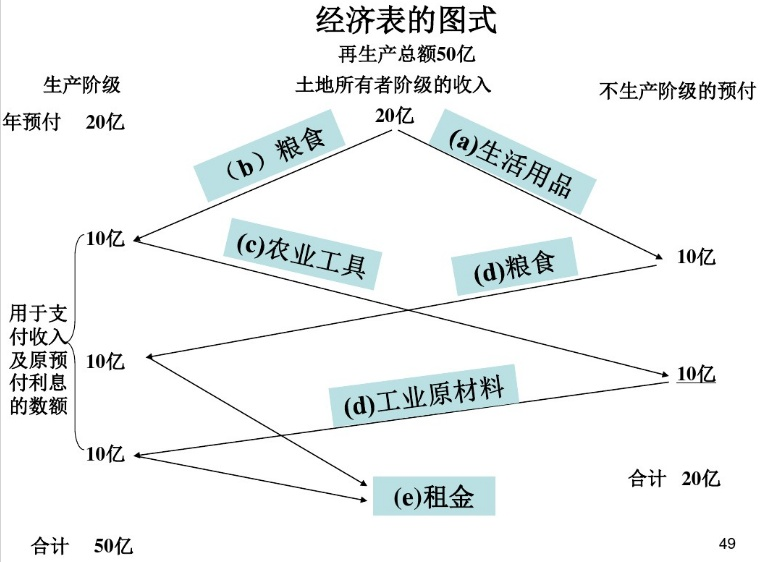
\includegraphics[width=\linewidth]{kuinai.jpg}
  \caption{\label{fig:label}摘自知乎 寒霜雪蝶 的文章 }
\end{figure}

重农主义者不仅就经济体不同部门之间的关系建立结论,而且试图量化它们的规模。在这一
方面,重农主义先于诺贝尔奖获得者瓦西里·里昂惕夫于20世纪30年代所提出的著名的“投
入——产出表”,并且先于以计量经济学家而知名的数量经济学家专业小组所做的工作。经济
表证明了经济体不同部门相互依赖的存在。

\subsection{重农主义经济政策}

重农主义者对微观经济理论的贡献不如他们对宏观经济理论的贡献那么大。他们认
为,\textbf{获得最大收益的愿望是人类经济活动的根本动机}。价格在市场中通过经济活动
而得以形成;价格的形成能够被加以研究,因为它受\textbf{独立于人类已知的自然法则}所
支配。他们的价格理论不连贯,但是他们推导\textbf{自由竞争导致最优价格};如果每个个
体都追求自己的私利,那么社会将从中受益。此外,他们认为,\textbf{净产品的唯一源泉
  是农业,据此推断税收负担将最终依赖于土地}。……重农主义者开始意识到在经济体不同
部门活动一体化过程中价格所起的作用。像更加敏感的重商主义者一样,他们认识到,看上
去在市场经济中独立经营的个人,实际上是在为其他人而经营,这些独立的活动通过价格体
制结合在一起。

重农主义者认为,存在一种比人类所设计的任何秩序都优越的自然秩序,所以,他们把经济
体想象成在很大程度上是自我规制的,并因此\textbf{拒绝重商主义体系所施加的控制。政
  府特有的任务是实行自由放任的政策——对事物不加干涉。}这一观点被斯密以及后来的经济
学家所领悟。

重农主义者认为,经济增长的主要障碍来自重商主义者对国内与国外贸易的规制政策。他们
尤其反对重商主义者的税收体制,提倡对土地征收单一税。

反对法国禁止谷物出口,反对对谷物价格控制。因为重农主义者没有预见到制造业的发展,
所以他们推断自由放任政策将引起法国农业的巨大增长,就像封建经济的小规模农业被大规
模农业所替代一样。因而,法国经济体的财富与权力也将增加。……重商主义者提倡鼓励贸
易顺差的政策——尤其是国际贸易形式的交换。重农主义者则认为净产品的源泉是农业(生
产,而不是交换),并主张自由放任会引起农业生产的增加,最终引致更大的经济增长。

\section{西班牙经济思想}

哥伦布1492年发现新大陆,西班牙成为强国,黄金大量流入造成西班牙国内价格水平上
升……货币数量论……

马丁·阿斯皮利奎塔的成就在于他能够观察到西班牙价格总水平的上升,并从通货膨胀很多可
能的原因中抽象出金银流入与价格上涨之间的关系。\textbf{货币数量论的脉络:阿斯皮利
  奎塔--马歇尔--弗里德曼。}

像其他经院哲学著作一样,路易斯·摩里纳关于公正与法律的著作本身就在关注发展中的经济
体的道德方面。他主张,在能够对任何一个特定市场作出道德判断之前,有必要了解特定的
市场事实上是如何实行的。……他精细陈述的16世纪的观点,即我们今天所称的\textbf{供
  需定理以及货币数量理论}。

像英国与法国后期重商主义一样,在西班牙重商主义末期,经济学家们很少倾向于支持政府
在对外贸易上的严格规制,而是\textbf{更多倾向于自由的经济思想}。彼得罗·罗德瑞库兹·康
姆庞曼斯伯爵是一位相当多产的经济学家。他认为\textbf{美洲流入到西班牙的金银具有可
  怕后果}。因为西班牙人能够比较便宜买到法国与英国的产品,所以,西班牙的生产能力就
不能像欧洲其他国家那样得到充分发展,这将最终导致金银从西班牙流向英法及低地国家。
康姆庞曼斯提倡给予外贸较大自由以及其他一些措施,这使得他既是一位重要的后期重商主
义者,也是一位早期的自由主义者。

\section{总结}

重商主义者和重农主义者公认经济体能够被正式加以研究。同时,他们发展抽象方法,也是
第一批模型构建者。……所以有充足的理由将重商主义者与重农主义者视为第一批经济理论
家。

威廉·配第在本质上是一个重商主义者,其重要性在于他最早试图将经济学置于经验观察之
中。斯密对政治算术的反对,以及获取相当精确数据的难题,使量化运动延迟了将近一百年。

就重商主义的死亡来说,可能没有比大卫·休谟的宣言总结得更好的了:“我由此要斗胆声
明,不仅作为一个人,而且作为一个英国人,我祈祷德国、西班牙、意大利甚至是法国自身
的商业繁荣昌盛。”
